\textbf{Ejemplo 3:}\\
Hallar el valor futuro de una serie de 30 pagos trimestrales de 25.000 COP c/u suponiendo una tasa del 24\% nominal anual mes vencido. Use el procedimiento para modificar los pagos.\\

\textbf{Solución}

La situación planteada en el problema es la siguiente:

Para poder  solucionar  el  problema  tiene que coincidir la periodicidad de liquidación de intereses (el período del valor de j) con la periodicidad de los pagos (el periodo de n), para llegar a esta coincidencia se cambian los pagos  de  trimestrales  a  mensuales,  entonces  un  pago  de 25.000 COP  deberá  ser reemplazado por tres pagos mensuales de R COP.

%La tabla ira centrada
\begin{center}
 \renewcommand{\arraystretch}{1.4}% Margenes de las celdas
 %Creación de la cuadricula de 3 columnas
 \begin{longtable}[H]{|c|c|c|}
  %Creamos una linea horizontal
  \hline
  %Definimos el color de la primera fila
  \rowcolor[HTML]{FFB183}
  %%%%% INICIO ASIGNACIÓN FECHA FOCAL %%%%%%%
  %%%%%%%%%% INICIO TITULO
  %Lo que se hace aquí es mezclar las 3 columnas en una sola
  \multicolumn{3}{|c|}{\cellcolor[HTML]{FFB183}\textbf{1. Asignación período focal}}\\ \hline
  \multicolumn{3}{|c|} {$pf_{1} = \textit{3 pmv}$}\\
  \multicolumn{3}{|c|}{$pf_{2} = \textit{30 ptv}\equiv\textit{90 pmv}$}\\ \hline
  %%%%%%%%%% FIN TITULO
  %%%%% INICIO DECLARACIÓN DE VARIABLES %%%%%%%
  %%%%%%%%%% INICIO TITULO
  %Lo que se hace aquí es mezclar las 3 columnas en una sola
  \multicolumn{3}{|c|}{\cellcolor[HTML]{FFB183}\textbf{2. Declaración de variables}}\\ \hline
  %%%%%%%%%% FIN TITULO
  %%%%%%%%%% INICIO DE MATEMÁTICAS
  %Cada & hace referencia al paso de la siguiente columna
  $\hspace{1.5 cm}R=25{.}000\,\,COP\hspace{1.5 cm}$ &  $\hspace{1 cm}n_1=\textit{3 pmv}\hspace{1 cm}$ & \\
  $j=24\% \textit{ namv}\hspace{0.1 cm}$ & $n_2=\textit{90 pmv}$ & $R_1=\,?\,\,COP$\\
  $i=2\%\textit{ pmv}$ & &\\
  \hline
  
  %%%%%%%%%% FIN DE MATEMÁTICAS
  %%%%% FIN DECLARACIÓN DE VARIABLES
  
  
  %%%%% INICIO FLUJO DE CAJA
  \rowcolor[HTML]{FFB183}
  \multicolumn{3}{|c|}{\cellcolor[HTML]{FFB183}\textbf{3. Diagrama de flujo de caja}}\\ \hline
  %Mezclamos 3 columnas y pondremos el dibujo
  %%%%%%%%%%%%% INSERCIÓN DE LA IMAGEN
  %Deberán descargar las imágenes respectivas del drive y pegarlas en la carpeta
  %n_capitulo/img/ejemplos/1/capitulo1ejemplo1.pdf  (el /1/ es el numero del ejemplo)
  \multicolumn{3}{|c|}{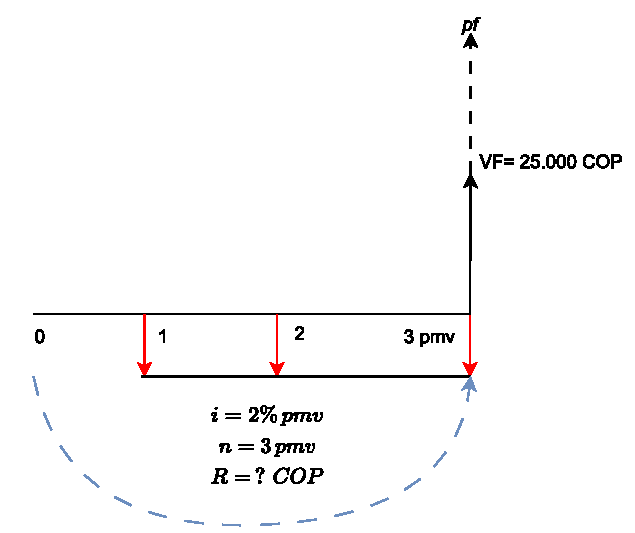
\includegraphics[trim=-5 -5 -5 -5 , max width=250px, max height=350px]{5_Capitulo/ejemplos/3/Capitulo5Ejemplo3-1.pdf}}\\
  \hline
  \multicolumn{3}{|c|}{ 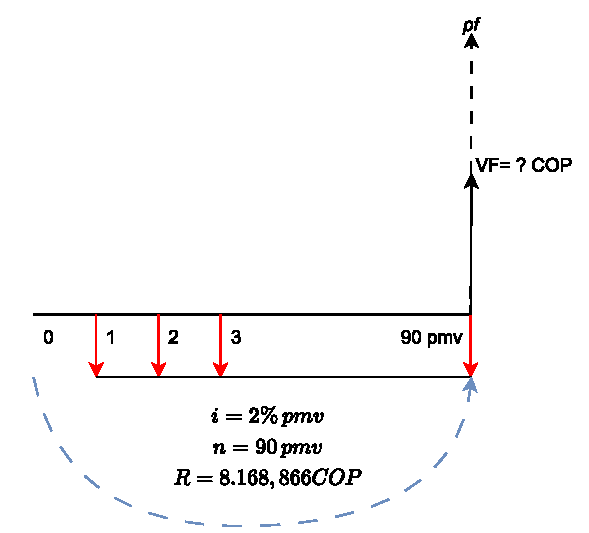
\includegraphics[trim=-5 -5 -5 -5 , max width=250px, max height=350px]{5_Capitulo/ejemplos/3/Capitulo5Ejemplo3-2.pdf}}\\ 
  \hline
  %%%%%%%%%%%%% FIN INSERCIÓN DE IMAGEN
  %%%%%FIN FLUJO DE CAJA
  
  
  
  %%%%% INICIO DECLARACIÓN FORMULAS
  %%%%%%%%%%% INICIO TITULO
  \rowcolor[HTML]{FFB183}
  \multicolumn{3}{|c|}{\cellcolor[HTML]{FFB183}\textbf{4. Declaración de fórmulas}}\\ \hline
  %%%%%%%%%%% FIN TITULO
  %%%%%%%%%%% INICIO MATEMÁTICAS
  
  \multicolumn{3}{|c|}{$VF=R(\frac{(1+i)^n-1}{i}) \hspace{0.4 cm} \textit{Valor futuro de una serie uniforme vencida}$}\\ \hline
  
  %%%%%%%%%% FIN MATEMÁTICAS
  %%%%%% INICIO DESARROLLO MATEMÁTICO
  \rowcolor[HTML]{FFB183}
  %%%%%%%%%%INICIO TITULO
  \multicolumn{3}{|c|}{\cellcolor[HTML]{FFB183}\textbf{5. Desarrollo matemático}}\\
  \hline
  %%%%%%%%%% FIN TITULO
  %%%%%%%%%% INICIO MATEMÁTICAS
  \multicolumn{3}{|c|}{$25{.}000\,\,COP=R(\frac{(1+0.02)^3-1}{0.02})\hspace{0.2 cm}\rightarrow \hspace{0.2 cm}R=\frac{25{.}000\,\,COP}{3,0604}\approx8{.}168,866\,\,COP$}\\
  \multicolumn{3}{|p{\textwidth}|}{Esto significa  que  cada  pago  de 25.000 COP podrá  ser  reemplazado  por  tres  pagos mensuales de  8.169 COP, de manera que resultarán 90 pagos mensuales en vez de los 30 trimestrales.}\\
  \multicolumn{3}{|c|}{$VF=8{.}168.87\,\,COP(\frac{(1+0.02)^{90}-1}{0.02})$}\\
  \hline
  
  
  %%%%%%%%%% FIN MATEMÁTICAS
  %%%%%% FIN DESARROLLO MATEMÁTICO
  %%%%%% INICIO RESPUESTA
  \rowcolor[HTML]{FFB183}
  %%%%%%%%%%INICIO TITULO
  \multicolumn{3}{|c|}{\cellcolor[HTML]{FFB183}\textbf{6. Respuesta}}                                                                                                                             \\ \hline
  %%%%%%%%%% FIN TITULO
  %%%%%%%%%% INICIO RESPUESTA MATEMÁTICA
  \multicolumn{3}{|c|}{El valor futuro de la serie de pagos es de ${VF=2{.}018{.}945,61\,\,COP}$}
  \begin{comment}
  \multicolumn{3}{|p{\textwidth}|}{
  $F_{4} = F_{5} = COP 21{.}610 $ .}
  \end{comment}
  \\ \hline
  %%%%%%%%%% FIN MATEMÁTICAS
  %%%%%% FIN RESPUESTA
 \end{longtable}
 %Se crean dos lineas en blanco para que no quede el siguiente texto tan pegado
 %\newline \newline %USARLO SI CREES QUE ES NECESARIO
\end{center}
%%%%%%%%%%%%%%%%%%%%%%%%%%FIN EJERCICIO 3 %%%%%%%%%%%%%%%%%%%%%%%%%%%
